\section{Suite TCP/IP}
    L'ISO-OSI è un modello di riferimento, nel senso che si suppone che i produttori di hardware e software seguino gli standard proposti per sviluppare i propri servizi. La \textbf{suite TCP/IP} è stata sviluppata quando il modello OSI non era ancora diventato uno standard, motivo per cui gli sorgono della disambiguità fra i due. Il TCP/IP, in effetti, segue l'ISO-OSI, e per ogni strato utilizza un protocollo diverso.

    \begin{center}
        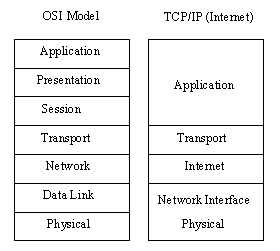
\includegraphics{images/TCP.png}
    \end{center}

    La suite TCP/IP permette il funzionamento di Internet. Si ispira all'ISO-OSI e ha una stratificazione a livelli. Ha 5 strati (4 se si accorpano lo strato fisico e quello di collegamento). Il TCP/IP non specifica, né per lo strato fisico, né per lo strato di collegamento, alcun protocollo. Si può usare qualsiasi protocollo previsto dall'hardware di rete. 

\subsection{Overview}
    Il protocollo che adempie alle funzionalità dello strato di rete è l'\textbf{Internet Protocol} (IP), che usa l'indirizzamento logico per la consegna di pacchetti da un nodo all'altro (datagram). Lo strato di rete non permette una consegna affidabile dei dati perché i datagram possono seguire strade diverse e quindi arrivare alla destinazione in ordine diverso da quello di spedizione, o addiritura duplicarsi o venire persi. 
    L'IP "\textit{fa del suo meglio}", senza però offrire garanzia alcuna. Ulteriori protocolli utilizzati nello strato di rete sono \textit{ARP} e \textit{RARP} (risoluzone indirizzi), \textit{ICMP} e \textit{IGMP}.

    \vspace{3mm}

    Lo stato di trasporto utilizza i protocolli \textit{UDP} (senza garanzie di consegna, implementata per necessità di celerità), \textit{TCP} (trasmissione affidabile) e \textit{SCTP} (per dati multimediali). L'UDP viene adoperato, ad esempio, per gli streaming su Teams: perdere un pacchetto in una conferenza non è chissà che problema, ma perdere un pacchetto durante una transazione bancaria lo è eccome. Per la transazione bancaria verrebbe utilizzato il TCP.

    \vspace{3mm}

    Lo strato applicativo, che include gli strati di presentazione e di sessione, si rifa in toto all'ISO-OSI. I "protocolli" in questo caso coincidono con i "programmi" utilizzati (posta elettronica, Web, etc).

    \vspace{3mm}

    Nella suite TCP/IP vengono impiegati quattro tipi di indirizzamento:

    \begin{itemize}
        \item 
            \textbf{Indirizzi fisici} (strato fisico e di collegamento), rappresentato dal MAC Address. E' cablato all'interno della scheda di rete, è una sequenza di 6 byte trascritti nell'interfaccia di rete.
        
        \item
            \textbf{Indirizzi logici} (strato di rete), rappresentato dall'IP Address. E' una sequenza di 4 byte in notazione decimale puntata. Ogni computer connesso ad Internet ha un indirizzo IP.
        
        \item
            \textbf{Indirizzi di porta }(strato di trasporto), rappresentato dai numeri di porta. Gli indirizzi IP e MAC sono necessari per far arrivare i dati al destinatario; tuttavia, su un singolo computer possono essere in esecuzione contemporaneamente più programmi: l'indirizzo di porta ci permette di determinare a quale programma inviare i dati. Le porte sono a 2 byte.
        
        \item
            \textbf{Indirizzi specifici} (strati applicativi), rappresentati da vari indirizzi, come l'indirizzo email
    \end{itemize}
